
%----------------------------------------------------------------------
\documentclass[xcolor=svgnames]{beamer} %, handout
\usetheme{lined}
\usepackage{array}
\usepackage{amsmath}
\usepackage{amssymb}
\usepackage{amsthm}
\usepackage{bbm}
\usepackage[utf8]{inputenc}
\usepackage[T1]{fontenc}
\usepackage{cmbright}   
\usepackage{times}
\usepackage{geometry}
\usepackage[spanish]{babel}
\usepackage{multicol}
\usepackage{tcolorbox}

\usepackage{algorithm2e}

%\usepackage{psfrag}
\usepackage{graphicx}
\usepackage{color}
\usepackage{floatflt}
\usepackage{fancybox}
\usepackage{tabularx}
%\usepackage[all]{xy}
\usepackage{color}

%\usepackage[most]{tcolorbox}


\theoremstyle{plain}
\newtheorem{definicion}{Definición}



\definecolor{redUnq}{rgb}{.7,.1,.1}
\definecolor{redUnq2}{rgb}{.5,.1,.3}

\mode<presentation>{
	%\usetheme{Boxes}
	%\usecolortheme[RGB={237,132,8}]{structure}
	%\usecolortheme[RGB={205,173,0}]{structure}
	\usecolortheme[RGB={100,10,10}]{structure}

	%\beamertemplateshadingbackground{SteelBlue!70}{Honeydew!10}
	%\usetheme{Warsaw}
	%\usecolortheme{default}
	\usetheme{Singapore}
	%\usetheme{Lined}
	%\usetheme[height=7mm]{Rochester} 
	\setbeamerfont{title}{shape=\bfseries,family=\rmfamily}
	%\usefonttheme[onlylarge]{structuresmallcapsserif}
	%\usefonttheme[onlysmall]{structurebold}
	\setbeamercolor{title}{fg=redUnq,bg=gray!40}
	\usefonttheme{professionalfonts}
	\setbeamercovered{highly dynamic}
	\setbeamercovered{transparent=10}
	\setbeamertemplate{navigation symbols}{}
	\colorlet{structure}{redUnq}

	\setbeamertemplate{frametitle}[default][left]
}

\definecolor{verzul}{rgb}{0, 0.5,0.5}

\renewcommand{\textbf}[1]{{\bfseries\textcolor{redUnq2}{#1}}}
\renewcommand{\emph}[1]{{\em\textcolor{redUnq2}{#1}}}

\setlength{\parindent}{0pt}
\theoremstyle{definition}
\newtheorem{ejem}{Ejemplo}
\newtheorem{defi}{Definición}
\newtheorem{ejer}{Ejercicio}
\newtheorem{prop}{Propiedad}
\newtheorem{lema}{Lema}
\newtheorem{teor}{Teorema}
\newtheorem{coro}{Corolario}

 

\newcommand{\Rset}{\mathbbmss{R}}
\newcommand{\Cset}{\mathbbmss{C}}
\newcommand{\PD}[2]{\frac{\partial #1}{\partial #2}}
\DeclareMathOperator{\tr}{tr}
\DeclareMathOperator{\adj}{adj}
\DeclareMathOperator{\rango}{rango}

\newenvironment{Boxedminipage}%
{\begin{Sbox}\begin{minipage}}%
{\end{minipage}\end{Sbox}\fbox{\TheSbox}}



\title{Métodos Numéricos - Clase 0}
  \logo{\includegraphics[scale=0.25]{logoUnq} }
\author{Ulises Bussi- Javier Portillo}
%\institute{\scalebox{2}{\includegraphics[scale=0.1]{mdp02.jpg}}} %{Departamento de Ciencia y Tecnología\\ Universidad Nacional de Quilmes\\ }
\date{ $1^\circ$ cuatrimestre 2020} 


%%%%%%%%% Para que al comenzar una section aparezca el Contenido
%\AtBeginSection[]
%{
%  \begin{frame}
%    \frametitle{Contenidos de la Presentación}
%    \tableofcontents[currentsection]
%  \end{frame}
%}




\begin{document} 


\begin{frame} %\thispagestyle{empty}
	\titlepage
\end{frame}


\begin{frame}
\frametitle{Usted está aqui} 

\begin{center}
\begin{itemize}
	\item Universidad Nacional de Quilmes.
	\begin{itemize}
		\item Departamento de Ciencia y Tecnología.
	\end{itemize}
	\item Bernal, Buenos Aires, Argentina.
	\item Marzo del año 2020.

	\item \begin{Large}
	\hspace{30pt}\textbf{Métodos Numéricos.}
	\end{Large}

	
\end{itemize}
\end{center}

\vspace{10pt}

La materia será dictada por \textbf{Ulises Bussi }y \textbf{Javier Portillo}.

Los \textbf{Miércoles de 18Hs a 22Hs} (carga horaria 4Hs semanales).

\end{frame}



\begin{frame}
\frametitle{Objetivos}
Los principales objetivos de la materia son:
\begin{itemize}
	\item Adquirir:
	\begin{itemize}
		\item Herramientas para la resolución de problemas.
		\item Capacidad de selección de un algoritmo adecuado para la resolución de un problema.
	\end{itemize}

	\item Entender ventajas y desventajas de:
	\begin{itemize}
		\item Algoritmos seleccionados.
		\item Métodos numéricos vs soluciones analíticas.
	\end{itemize}
	\item Ganar manejo de:
	\begin{itemize}
		\item Software específico de cálculo numérico.
		\item Redacción de informes.
		\item Presentaciones.
	\end{itemize}

  \end{itemize}
\end{frame}


\begin{frame}
	\frametitle{Cursada}
	La cursada tendrá aproximadamente 12 clases de 4 Hs ($\sim$ 2 teóricas + 2 prácticas), una por semana.


	\textbf{Evaluación:}
	\begin{itemize}
		\item Un parcial teórico.
		\item Dos trabajos prácticos.
		\item Un trabajo final de materia.
		\item Un examen final (en caso de no promocionar).
	\end{itemize}


\begin{tcolorbox}
\begin{small}


 \textbf{Régimen de aprobación:}

	\begin{algorithm}	[H]
		aprobado = True;\\
		\For{nota in notas}{
			aprobado $\&=$ (nota$>$6);
		}
	promedio = mean(notas);\\
	\Return{ aprobado $\&$ (promedio>7)}
	\end{algorithm}	 
\end{small}
\end{tcolorbox}

\end{frame}




\begin{frame}
	\frametitle{Contenidos de la materia}

	\begin{itemize}
		\item \textbf{Unidad 0-1:} Básicas de métodos numéricos y programación.
		\item \textbf{Unidad 2:} Resolución de Ecuaciones Lineales y factorización.
		\item \textbf{Unidad 3:} Resolución de Ecuaciones No Lineales.
		\item \textbf{Unidad 4:} Aproximación de funciones, Cálculo numérico (integración y derivación)
		\item \textbf{Unidad 5:} Resolución de Ecuaciones Diferenciales Lineales.
	\end{itemize}
\end{frame}



\begin{frame}
	\frametitle{Bibliografía Recomendada}
	\begin{itemize}
		\item Burden, R. L., $\&$ Faires, J. D. (1988). Numerical analysis.
		\item Chapra, S. C., $\&$ Canale, R. P. (2010). Numerical methods for engineers
		\item https://la.mathworks.com/
	\end{itemize}
\end{frame}









\begin{frame}
\frametitle{¿Por qué Métodos Numéricos?}
\begin{tcolorbox}
	\begin{defi}
		Los métodos numéricos son procedimientos que permiten obtener, de forma aproximada, solución a problemas, por medio de la aplicación de algoritmos
	\end{defi}
\end{tcolorbox}


Son una herramienta poderosa a la hora de resolver problemas porque permiten:
\begin{itemize}
	\item Resolver problemas rápidamente.
	\item Manejo de dimensionalidad grande.
	\item Encontrar soluciones a problemas que no pueden resolverse analíticamente.
\end{itemize}

\end{frame}


\begin{frame}
\frametitle{¿Por qué \textbf{NO} Métodos Numéricos?}

En general sirven, siempre y cuando, podamos elegir y aplicar bien el método correcto.
\vspace{40pt}

{\centering
No conviene aplicarlos en los siguientes casos:
\begin{itemize}
	\item Carencia de criterio.
\end{itemize}}



\end{frame}


\begin{frame}
\frametitle{¿Por qué \textbf{NO} Métodos Numéricos?}



Un método no bien elegido puede traer consigo problemas:
\vspace{40pt}

\begin{itemize}
\item Solución incorrecta.
\item Errores no despreciables en los resultados.
\item Grandes costos computacionales.
\end{itemize}


\end{frame}


\begin{frame}
\frametitle{Herramientas}
\textbf{Software}

Durante la cursada, vamos a trabajar con \textbf{Matlab} (por defecto, pero se puede usar cualquier otro( I.E. Octave, Python, Julia, R?¿).


\textbf{Conocimientos previos}

\begin{itemize}
\item Algorítmos y programación.
\item Análisis I y II. (Taylor, ecuaciones diferenciales)
\item Algebra Lineal. (nociones matriz, un determinante, un cambio de base. Polinomio Característico, Autovalores y Autovectores.)
\end{itemize}

\end{frame}





%
%\begin{frame}
%\frametitle{Contenidos de la presentación}
%\tableofcontents%[pausesections]
%\end{frame}
%
%\section{Introducción}
%
%
%\begin{frame}
%			\frametitle{Introducción}
%			Robótica móvil: \vspace{1.1cm}
%			
%	\begin{minipage}{.45\linewidth}
%		Integración de:
%		\begin{itemize}
%		\item Electrónica
%		\item Mecánica
%		\item Física
%		\item Programación
%		\item Control
%		\end{itemize}			
%	\end{minipage}
%	\begin{minipage}{.45\linewidth}
%		\vspace{-.5cm}Usos en:
%		\begin{itemize}
%        \item Transporte
%		\item Doméstico	        
%        \item Industria
%        \item Agricultura
%		\end{itemize}	
%	\end{minipage}
%\end{frame}
%
%
%
%
%\begin{frame}
%			\frametitle{Introducción}
%	La robótica móvil en agricultura: creciente aplicación.\vspace{.5cm}
%	
%	\begin{minipage}{.4\linewidth}
%		\begin{itemize}
%		\item[-] Permite reemplazar personas en trabajos de riesgo.
%		\item[-] Optimizar el uso de recursos.
%	\end{itemize}
%	\end{minipage}
%	\begin{minipage}{.55\linewidth}
%		    \centering
%		    \includegraphics[width=.8\linewidth]{Imgs/robotINTA.png}
%	
%	\end{minipage}	\vspace{.3cm}	\pause
%
%\begin{tcolorbox}[colback=blue!5!white,colframe=blue!75!black]
% Se propone evaluar el desempeño del uso de un EKF en dos estrategias de control para lograr seguimiento de trayectoria aun en presencia de ruido y sin contar con la medición total del estado. 
%\end{tcolorbox}
%
%
%\end{frame}
%
%%\begin{frame}
%%			\frametitle{Introducción}
%%Se propone evaluar el desempeño del uso de un EKF en dos estrategias de control para lograr seguimiento de trayectoria aun en presencia de ruido y sin contar con la medición total del estado.
%
%%	Se propone utilizar sensores de posición para realizar seguimiento de trayectorias.	
%%	A pequeña escala:
%%	
%%	\hspace{2cm} Posicionador ultrasónico ("GPS de interior" ) 
%%	
%%\begin{minipage}{.6\linewidth}
%%	\centering	
%%	\includegraphics[width=.8\linewidth]{Imgs/gpsInt.jpg}
%%\end{minipage}	
%%\begin{minipage}{.35\linewidth}
%%	$\pm 2 cm$ de error
%%\end{minipage}
%%	
%
%%\end{frame}
%
%
%%\begin{frame}
%%			\frametitle{Introducción}
%%Robots móviles de rueda ¿Por qué?\vspace{1cm}
%%
%%\begin{itemize}
%%	\item Eficiencia
%%	\item	Simplicidad
%%	\item Múltiples aplicaciones
%%\end{itemize}
%%\end{frame}
%
%
%\section{Descripción de la Plataforma Móvil}
%
%\begin{frame}
%  \frametitle{Descripción de la Plataforma Móvil}
%  \begin{itemize}
%  \item  Robot Móvil de tracción diferencial de tres ruedas
%
%\vspace{0.5cm}
%\begin{figure}[h]
%  \begin{minipage}{0.50\linewidth}
%    \centering
%    \includegraphics[width=1.07\linewidth]{Imgs/foto.jpg}
%  \end{minipage}
%  \begin{minipage}{0.49\linewidth}
%    \begin{itemize}
%    \item 2 Motores de CC \vspace{-0.1cm}
%    \item Posicionador ultrasónico (GPS indoor)\vspace{-0.1cm}
%    \item PC portatil
%    \end{itemize}
%  \end{minipage}
%\end{figure}
%  \end{itemize}
%\end{frame}
%\begin{frame}
%  \frametitle{Modelo Matemático}
%
%  \begin{minipage}{0.54\linewidth}
%    \begin{equation*}
%\begin{bmatrix}
%\dot{x} \\
%\dot{y} \\
%\dot{\theta}
%\end{bmatrix} = \begin{bmatrix}
%\cos\theta	&	0 \\
%\sen\theta	&	0 \\
%	0		&	1
%\end{bmatrix} \begin{bmatrix}
%V	\\
%W
%\end{bmatrix}, 
%\end{equation*}
%\end{minipage}
%\begin{minipage}{0.44\linewidth}
%      \begin{center}
%      \scalebox{0.6}{\input{Imgs/robotin.pdf_t}}
%    \end{center}
%  \end{minipage}
%
%\begin{itemize}
%\item \emph{$V$} velocidad tangencial $V = \dfrac{v_d + v_i}{2}$,
%  donde   $v_i$ y $v_d$ son las velocidades izquierda y derecha respectivamente.
%\item \emph{$W$} La velocidad angular $W = \dfrac{v_d - v_i}{L} $.
%\end{itemize}
%
%\end{frame}
%
%\section{Estrategias de Control}
%\subsection{Gerneración de Trayectoria}
%
%\begin{frame}
%  \frametitle{Generación de Trayectoria}
%Se parte desde una imagen digital con los obstáculos 
%    identificados
%
%\begin{minipage}{0.55\linewidth}
%  \begin{itemize}
%   \item Se reemplazan por circunferencias de un radio $r=r_o+ r_p+
%    r_s$
%  \item Se genera la trayectoria como una linea recta entre el punto
%    inicial y final, unida con secciones circunferencias que rodeen
%    los obstáculos, eligiendo el menor de los arcos 
%  \end{itemize}
%\end{minipage}
%  \begin{minipage}{0.44\linewidth}
%    \begin{figure}[h]
%      \begin{center}        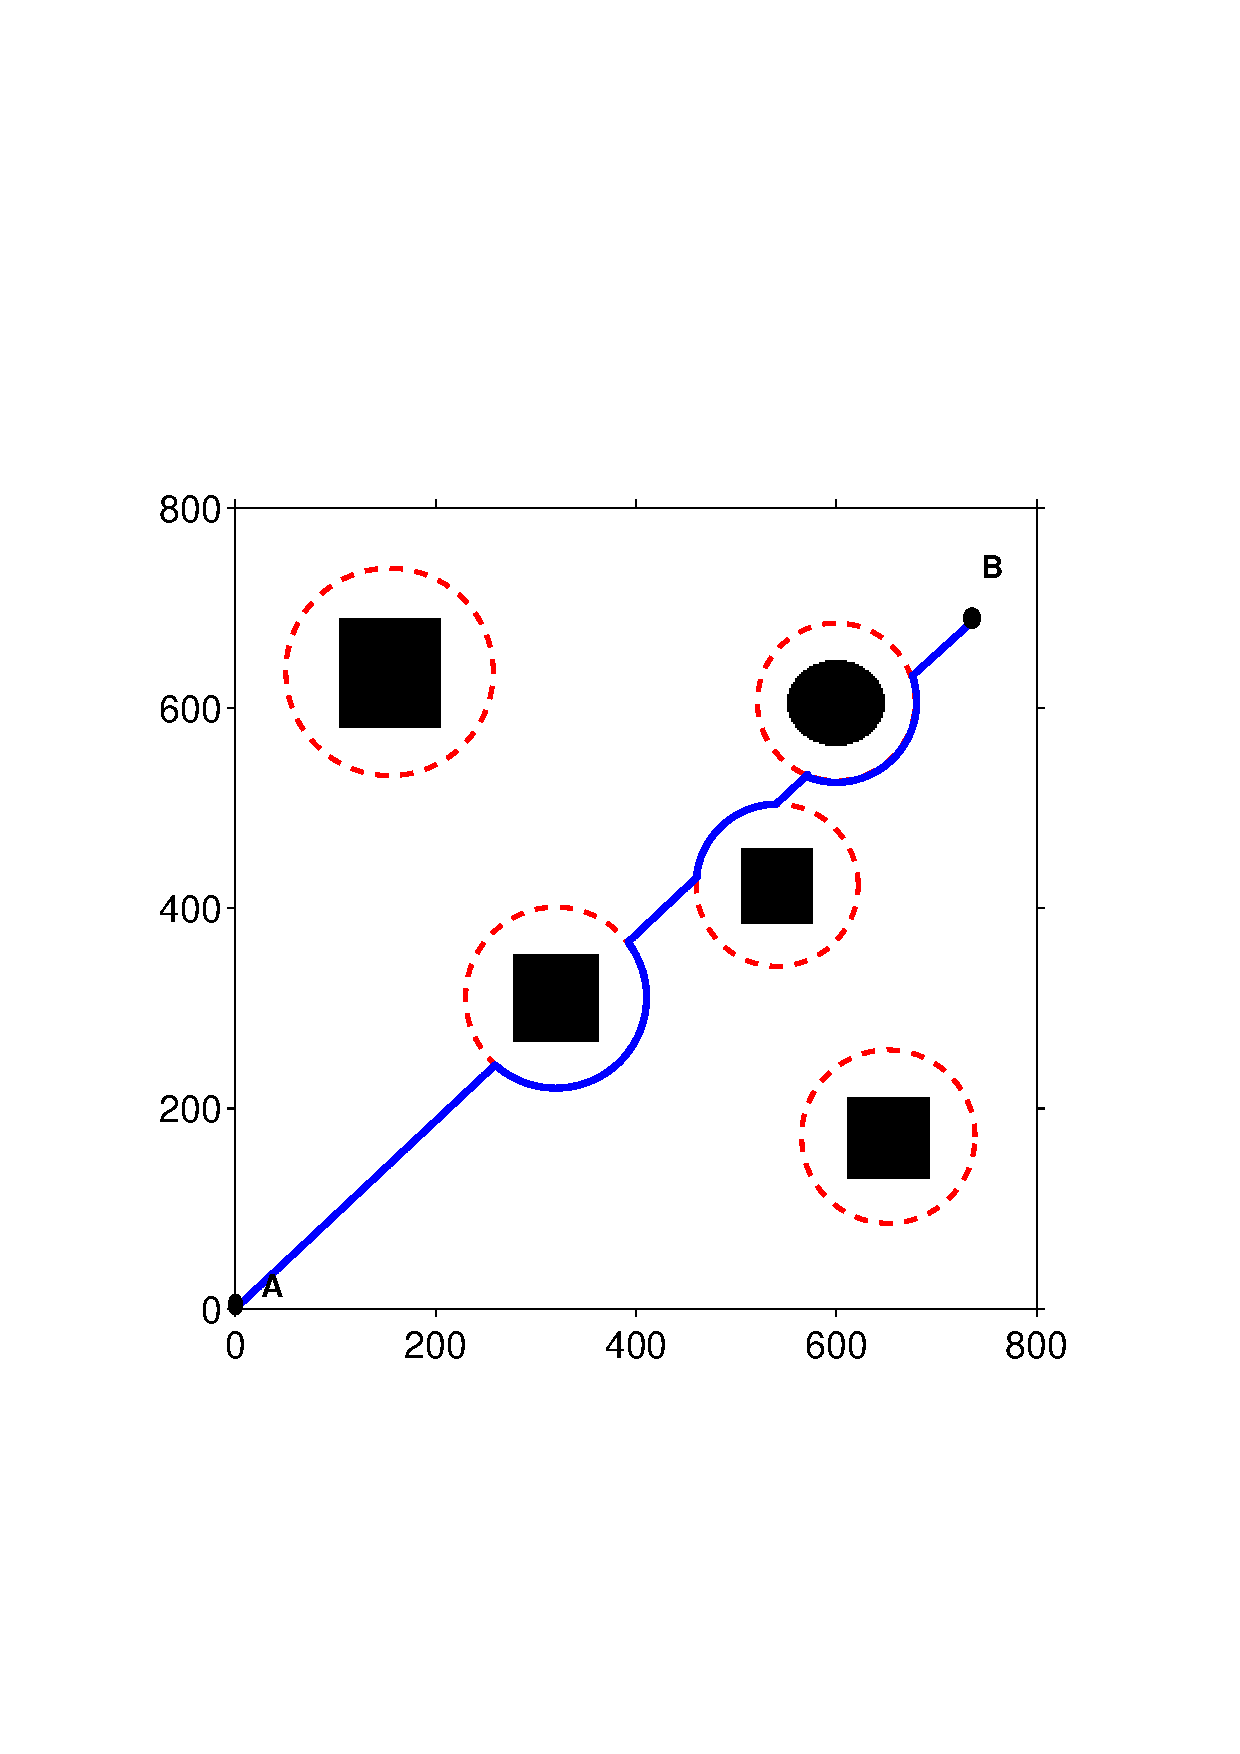
\includegraphics[width=1.2\linewidth]{Imgs/TrayectoriaGenerada_PresentacionRpic.pdf}  
%      \end{center}
%    \end{figure}
%  \end{minipage}
%
%
%\end{frame}
%
%\begin{frame}
%  \frametitle{Modelo matemático en variables del error}
%  Dado que el objetivo de control es seguir trayectorias, se propone
%  
%
%  \begin{minipage}{0.59\linewidth}
%\small{    \begin{equation*}
%      \begin{bmatrix}
%        x_e \\
%        y_e \\
%        \theta_e
%      \end{bmatrix} = \begin{bmatrix}
%        \cos \theta & \sen \theta & 0 \\
%        -\sen \theta & \cos \theta & 0 \\
%        0 & 0 & 1
%      \end{bmatrix}\begin{bmatrix}
%        x_{r}-x \\
%        y_{r}-y \\
%        \theta_{r}-\theta
%      \end{bmatrix},
%    \end{equation*}}
%  \end{minipage}
%\begin{minipage}{0.4\linewidth}
%  \begin{figure}[h!]
%    \centering \scalebox{0.7}{\input{Imgs/Coord_error.pdf_t}}
%    % \caption{Descripción de las variables del
%    %   error$(x_e,y_e,\theta_e)$, en función del estado real
%    %   $(x,y,\theta)$ y el estado de referencia $(x_r,y_r,\theta_r)$}
%    % \label{fig:Var_error}
%  \end{figure}
%\end{minipage}
%\pause
%De esta forma,
%\small{
%\begin{equation*}
%\begin{bmatrix}
% \dot{x}_e \\
% \dot{y}_e \\
% \dot{\theta}_e
%\end{bmatrix} = \begin{bmatrix}
% y_e	& -1	\\
%-x_e	& 0		\\
%-1		& 0		\\
%\end{bmatrix}\begin{bmatrix}
%W \\
%V \\
%\end{bmatrix} +\begin{bmatrix}
%V_{r} \cos \theta_e \\
%V_{r} \sen \theta_e \\
%W_{r}
%\end{bmatrix} \label{eq:dinError}
%\end{equation*}}
%donde $V_{r}$ y $W_{r}$ son las entradas de referencia del
%sistema que generan la trayectoria deseada.
%
%\end{frame}
%
% \subsection{Control Basado en Integración Trapezoidal}
%
%
%
%\begin{frame}
%  \frametitle{Control Basado en Integración Trapezoidal}
%  Se considera el problema de control a partir de la discretización de
%  la ecuación diferencial. 
%  \begin{equation*}
%    \mathbf{x}_{n+1} = \mathbf{x}_{n} + \int_{t_n}^{t_{n+1}}
%    f(\mathbf{x},\mathbf{u}) dt
%  \end{equation*}
%
% Que aproximando la integral por el método trapezoidal:
%   \begin{equation*}
%   \mathbf{x}_{n+1} \approx \mathbf{x}_{n} + \frac{T}{2} \left [ f(\mathbf{x}_{n+1},\mathbf{u}_{n+1}) +
% f(\mathbf{x}_{n},\mathbf{u}_{n})  \right ]
% \end{equation*}
%
%De donde puede calcularse  $\mathbf{u}_{n}$ y
% $\mathbf{u}_{n+1}$ tal que $\mathbf{x}_{n+1} = \mathbf{x}_{deseado}$ 
%\end{frame}
%
%\begin{frame}
% \frametitle{Control Basado en Integración Trapezoidal} 
%
%Aplicándolo al modelo en variables del error \vspace{-.2cm}
%
%\footnotesize{
%\begin{equation*}  \label{eq:4}
%\begin{bmatrix}
%	1	& \hspace{-0.2cm}	1	&\hspace{-0.2cm}
%        -y_{e_n}	& \hspace{-0.2cm}	-y_{d{e_{n+1}}}	\\
%	0	&\hspace{-0.2cm}	0	&\hspace{-0.2cm}
%        x_{e_n}	&	\hspace{-0.2cm} x_{d{e_{n+1}}}	\\
%	0	&\hspace{-0.2cm}	0 	&
%        \hspace{-0.2cm} 1		&\hspace{-0.2cm}	1			\\
%\end{bmatrix} \begin{bmatrix}
%V_n\\
%V_{n+1}\\
%W_n\\
%W_{n+1}
%\end{bmatrix} = 
% \begin{bmatrix}
%-\cfrac{2 }{T}( x_{de_{n+1}} - x_{e_n}) + V_{r_n} \cos \theta_{e_n}+V_{r_{n+1}} \cos \theta_{d_{e_{n+1}}}\\
%-\cfrac{2}{T} (y_{de_{n+1}} - y_{e_n}) + V_{r_n} \sen \theta_{e_n}+V_{r_{n+1}} \sen \theta_{d{e_{n+1}}}\\
%-\cfrac{2}{T} (\theta_{de_{n+1}} - \theta_{e_n})+ W_{r_n} +W_{r_{n+1}}
%\end{bmatrix}
%\end{equation*}}
%donde $x_{de_{n+1}}$ y $y_{de_{n+1}}$ son el error deseado
%en $n+1$. La solución de mínima norma: 
%
%%original 0.45, 2 cols
%\begin{minipage}{0.45\linewidth}
%\raggedright
%  \begin{equation*}
%    \begin{bmatrix} 
%      V_n \\
%      V_{n+1}\\
%      W_n \\
%      W_{n+1}
%    \end{bmatrix}=\begin{bmatrix}
%      \frac{a_1}{2}\\
%      \frac{a_1}{2}\\
%      a_2\\
%      a_3
%    \end{bmatrix}
%  \end{equation*} 
%\end{minipage} \pause $\rightarrow \quad$ 
%\begin{minipage}{0.45\linewidth}
%  \begin{align*}
%    a_1 &= \frac{b_2-b_3 x_{e_n}}{x_{de_{n+1}}- x_{e_n}}\\
%    a_2 &= b_3 - W_{n+1} \\
%    a_3 &= b_1 + y_{e_n} W_{n+1}+ y_{e_n} W_n
%  \end{align*}
%  \end{minipage}  
%  
%   donde $b_1$, $b_2$ y $b_3$ son las componentes del vector del
%   miembro derecho del sistema de ecuaciones
%\end{frame}
%
%\begin{frame}
%			 \frametitle{Control Basado en Integración Trapezoidal}
%  \begin{equation*}
%  \begin{split}
%    V_n & =  k_V \dfrac{a_1}{2}\vspace{0.25cm}\\
%    W_n & = k_W a_2
%  \end{split}
%\end{equation*}
%con parámetros de diseño $0 <  k_V \leq 1$ y $0<k_W\leq 1$ para  garantizar la estabilidad y ajustar la dinámica del lazo cerrado.
%
%\end{frame}
%
% \subsection{Control Basado en Lyapunov}
%
%	
% \begin{frame}
%   \frametitle{Control Basado en Lyapunov}
%   Se proponen una acción de control y una función tal que se cumplan
%   las condiciones del Teorema de estabilidad de Lyapunov: \vspace{-1cm}
%
% \begin{equation*}
%   \begin{split}
%     V &= Vr \cos \theta_e + k_1 x_e \\
%     W &=  Wr + k_2 y_e Vr + k_3 V_{r} \sen \theta_e
% 	\end{split}  
% \end{equation*}
%
% \begin{equation*}
% V(x_e,y_e,\theta_e) = \frac{( x_e^2 + y_e^2 )}{2} + \frac{1}{k_2} (1 - \cos \theta_e) >0
% \end{equation*}
% 
% con $k_2 > 0$
%\end{frame}
%
%\begin{frame}
%	\frametitle{Control Basado en Lyapunov}
%	Calculando la derivada de la función:
%	\begin{equation*}
% 		\dot V(x_e,y_e,\theta_e)= -k_1 x_e^2 - \frac{k_3}{k_2} V_{r}\sen
% 		^2 \theta_e 
% 	\end{equation*}
% 	Es menor que $0$ si $k_1>0$ y $k_3>0$. $\rightarrow$ \textbf{El equilibrio es estable.}\vspace{.5cm}
% 	
% 	
% 	\begin{minipage}{0.35\linewidth}
%		 	Para demosrar la estabilidad asintótica, se propone linealizar alrededor del equilibrio: 	
% 	\end{minipage}
%	\begin{minipage}{0.55\linewidth}
%	 	\begin{equation*}
%	  	A=
%  		\begin{bmatrix}
%    		-k_1 & W_r & 0\\-W_r & 0 & V_r\\ 0 &-k_2 V_r & -k_3 V_r
%  		\end{bmatrix}
%		\end{equation*}
%	\end{minipage}\vspace{.5cm}
% 	
%	Por criterio de Routh-Hurwitz, se garantiza que $A$ tiene sus autovalores  con parte real	negativa. $\rightarrow$ \textbf{Estabilidad asintótica}
%
% \end{frame}
%
% \subsection{Filtro de Kalman Extendido}
%
% \begin{frame}
%   \frametitle{Filtro de Kalman Extendido -EKF-}
%   La estimación de la orientación:
%	\begin{equation*}
%		\dot{\theta} = W \rightarrow \theta_{k+1} \approx \theta_k+W_k T
%	\end{equation*}	  	
%	\pause
%  	Se propone utilizar EKF para filtrar la información de los sensores y
%  	estimar el estado no medible. 
%
%	El sistema con ruido:
%  	\begin{equation*}
%	   \begin{split}
%    	 \mathbf{x}_{k+1} &= f(\mathbf{x}_k, \mathbf{u}_k) +\mathbf{ q}_k\\
%     	 \mathbf{y}_k & = h(\mathbf{x}_k, \mathbf{u_k}) + \mathbf{r}_k
%   	   \end{split}
% 	\end{equation*}
%  	con $E(\mathbf{q}^T_k \mathbf{q}_k)= Q$, $E(\mathbf{r}_k^T
% 	\mathbf{r}_k)=R$ y $E(\mathbf{q}_j^T\mathbf{r}_k)=0$, donde $Q$, $R$ son las matrices de covarianza.
% \end{frame}
%
%
%
%\begin{frame}
%   			\frametitle{Filtro de Kalman Extendido -EKF-} \vspace{-.5cm	}
% Cuenta con dos etapas:\vspace{.5cm}
% 
%
% \begin{minipage}{0.48\linewidth}
% 	Predicción:
% 	\begin{equation*}	
% 		\begin{split}
% 		\check {\mathbf{x}}_{k+1} & = f(\hat{\mathbf{x}}_k, \mathbf{u}_k)\\
%	 	\check {\mathbf{y}}_{k+1} & = h(\check{\mathbf{x}}_{k+1},\mathbf{u_{k+1}}) \\
% 		\check P_{k+1} & =  F_{x_{k}} \hat P_k F_{x_{k}}^T + Q\\
%		K_{k+1} & =  \check P_{k+1} H_{X_{k+1}}^T (H_{X_{k}} \check P_{k+1} H_{X_{k}}^T + R)^{-1} 
% 		\end{split}  
% 	\end{equation*}
% \end{minipage}
% \begin{minipage}{0.48\linewidth}
% \vspace{-1.2cm}
% 	Estimación:
% 	\begin{equation*}
% 		\begin{split}
% 		\hat {\mathbf{x}}_{k+1} & =  \check {\mathbf{x}}_{k+1} + K_{k+1} (\mathbf{y}_{k+1} - 						\check{\mathbf{y}}_{k+1} ) \\
% 		\hat P_{k+1} & =  \check P_{k+1} -K_{k+1} H_{X_{k+1}} \check P_{k+1} \\
% 		\end{split} 
% 	\end{equation*}
% \end{minipage}
%
%\end{frame}
%
%
%
%
%
%
%\section{Resultados en Simulación}
%\begin{frame}
%			\frametitle{Resultados en Simulación}
%	Se realizan simulaciones de las dos estrategias de control descritas con las siguiente consideración:
%  	\begin{itemize}
%  		\item Las acciones de control están limitadas $0\leq V\leq 6$ en  $cm/s$ y
%   		$-0.3 \leq W \leq 0.3$ en $ rad/s$
%	 \end{itemize}
%	 
%	Se buscan los siguientes objetivos:	 
%	 \begin{itemize}
%		 \item Comparar el EKF contra un estimador basado en modelo	 
%		 \item Encontrar el seguimiento de la trayectoria
%		 \item Encontrar la convergencia del estimador basado en EKF.
%	\end{itemize}
% \end{frame}
%
%	
%
%\begin{frame}
%			\frametitle{Resultados en Simulación: Integración Trapezoidal}\vspace{-1cm}
%	\begin{minipage}{.35\linewidth}
%   		Para el método basado en integración trapezoidal, con 
%	    $ k_V = 0.02$ y $ k_W= 0.2 $ \vspace{3cm}
% 	\end{minipage}
% 	\begin{minipage}{.6\linewidth}
% 	\vspace{.9cm}
%   		\begin{figure}
%     		\begin{center}
%       			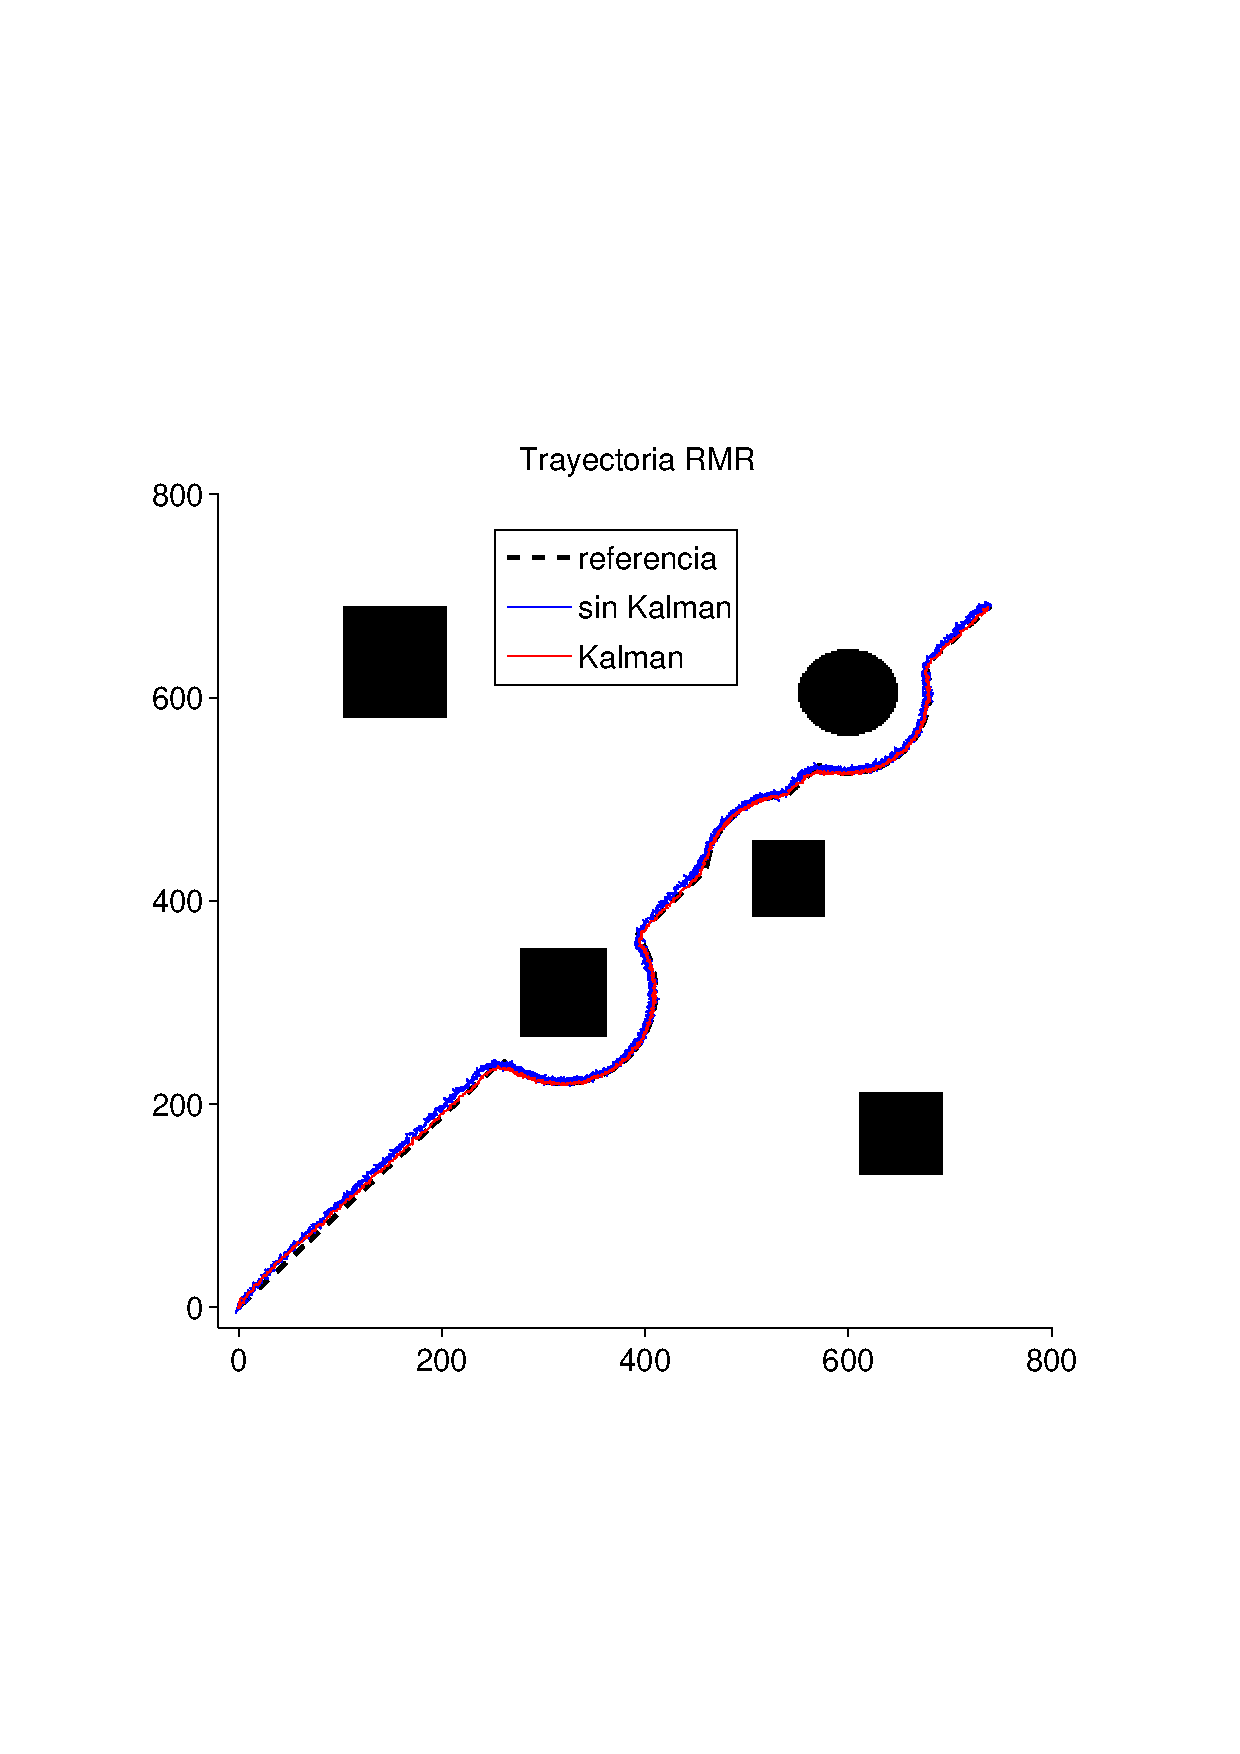
\includegraphics[width=1\linewidth]{Imgs/TrayNum.pdf}
%		    \end{center}
%   		\end{figure}
% 	\end{minipage}
%\end{frame}
%
%
%\begin{frame}
%   			\frametitle{Resultados en Simulación: Integración Trapezoidal}\vspace{.4cm}
%	\begin{minipage}{.35\linewidth}
%    	Para el método basado en integración trapezoidal, con 
%    	$ k_V = 0.02$ y $ k_W= 0.2 $ \vspace{3cm}
% 	\end{minipage} \vspace{-3.3cm}
%%	\begin{minipage}{.6\linewidth}
%   		\begin{figure}
%     		\begin{center}
%       			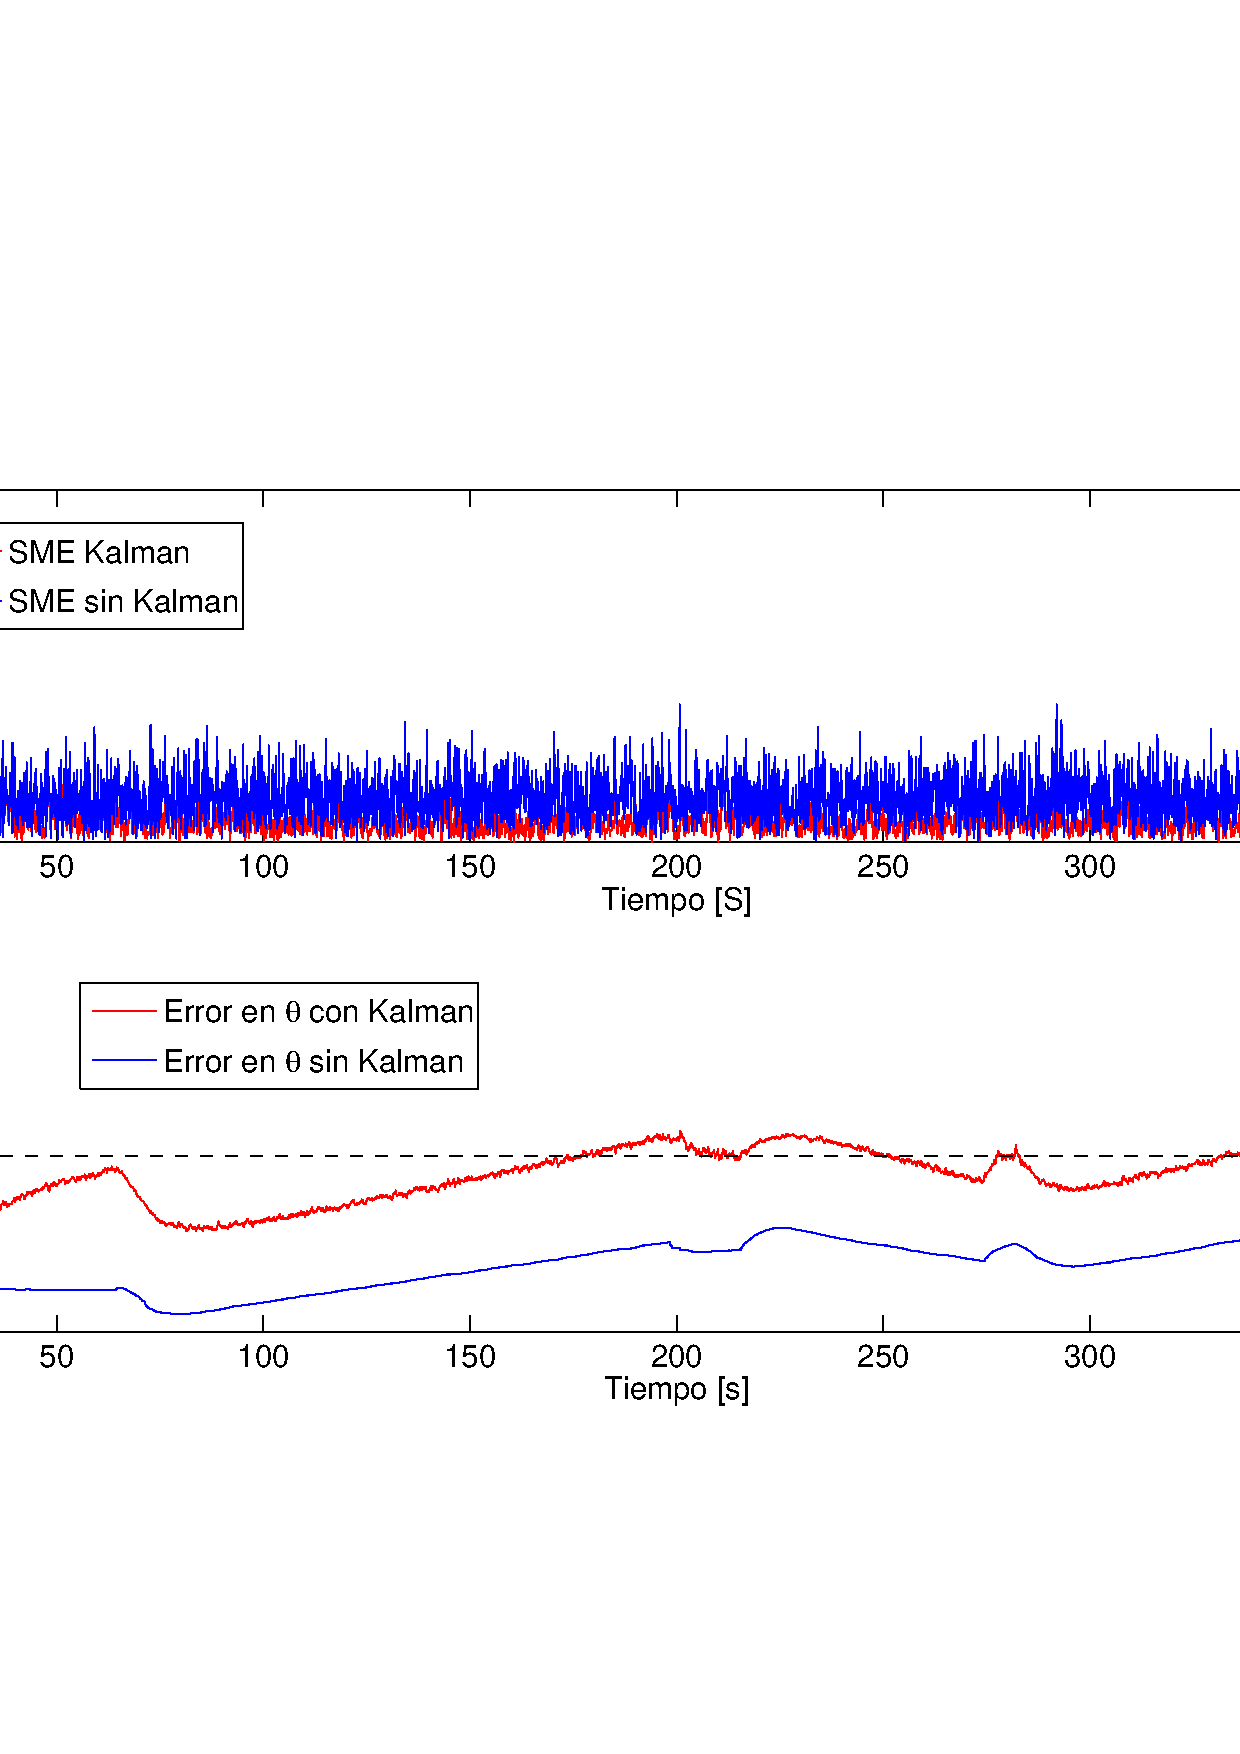
\includegraphics[width=.9\linewidth]{Imgs/sme_Num.pdf}
%     		\end{center}
%	   	\end{figure}
%%	 \end{minipage}
%\end{frame}
%
%
%
%\begin{frame}
%   			\frametitle{Resultados en Simulación: Lyapunov}\vspace{-1cm}
%	\begin{minipage}{.35\linewidth}
%   		Para el método basado en Lyapunov, con 
%	    $ k_1 = 1$, $k_2 =0.5$  y $ k_3= 2 $ \vspace{3cm}
% 	\end{minipage}
% 	\begin{minipage}{.6\linewidth}
%	\vspace{.9cm}   	
%   		\begin{figure}
%     		\begin{center}
% 	      		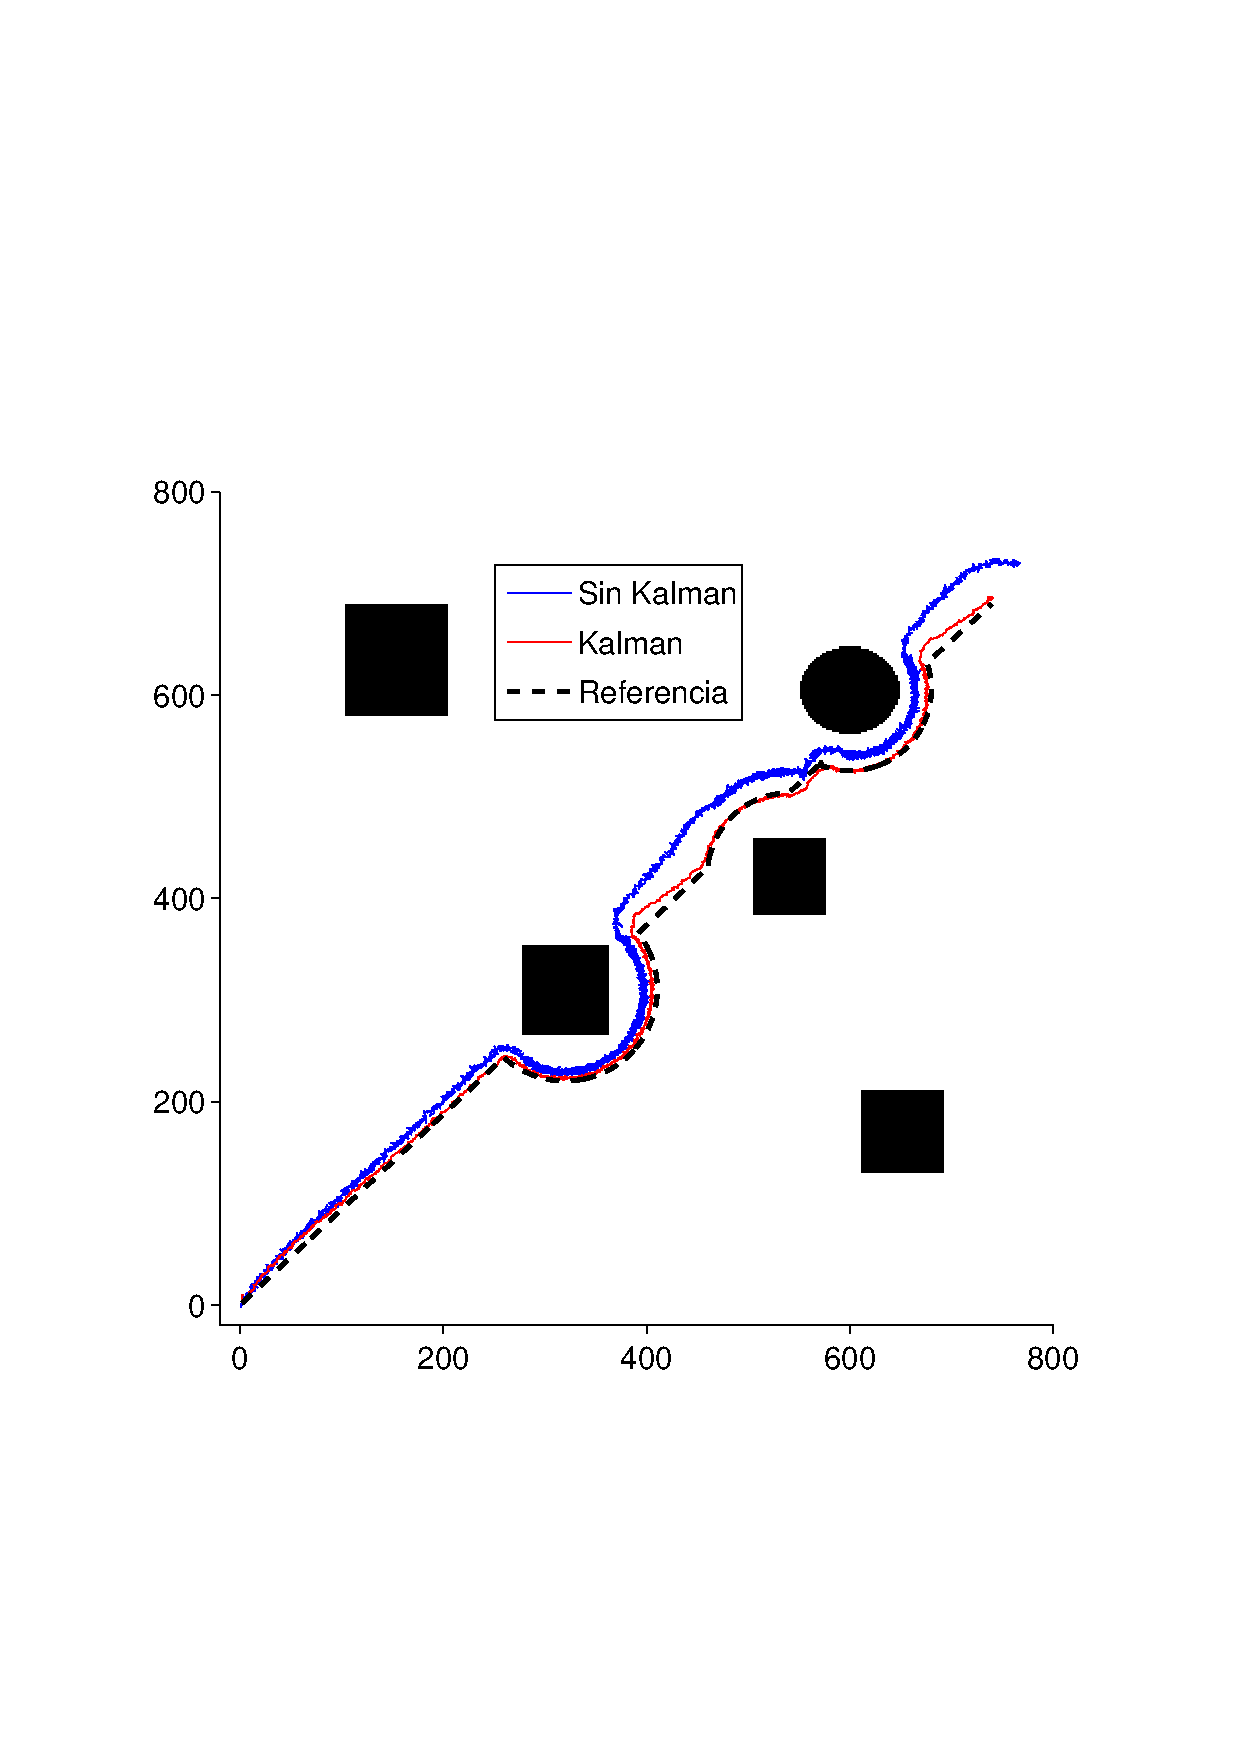
\includegraphics[width=1\linewidth]{Imgs/trayLyap.pdf}
%     		\end{center}
%   		\end{figure}
% 	\end{minipage}
%\end{frame}
%
%\begin{frame}
%%		\frametitle{Resultados en Simulación: Integración Trapezoidal}\vspace{.4cm}
%%	\begin{minipage}{.35\linewidth}
%%    	Para el método basado en integración trapezoidal, con 
%%    	$ k_V = 0.02$ y $ k_W= 0.2 $ \vspace{3cm}
%% 	\end{minipage} \vspace{-3.3cm}
%%%	\begin{minipage}{.6\linewidth}
%%   		\begin{figure}
%%     		\begin{center}
%%       			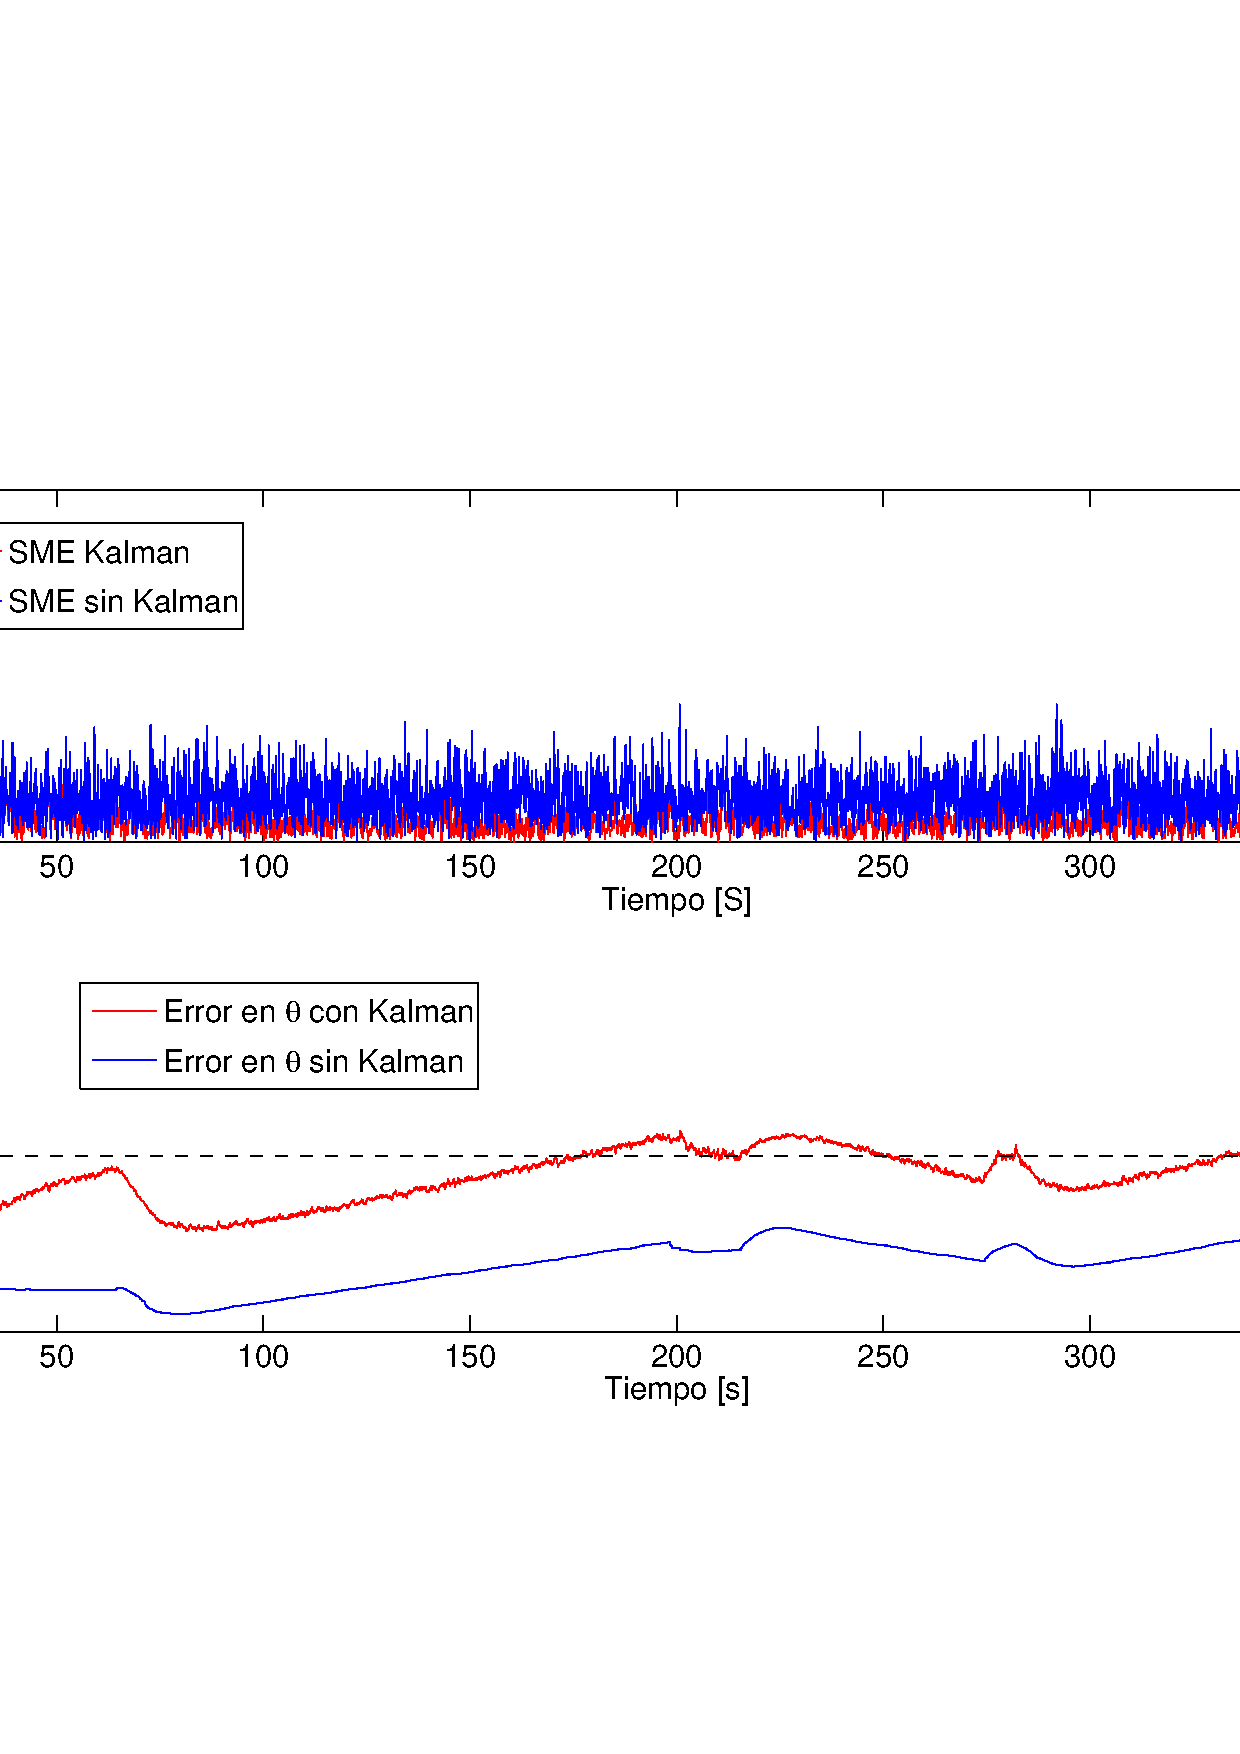
\includegraphics[width=.9\linewidth]{Imgs/sme_Num.pdf}
%%     		\end{center}
%%	   	\end{figure}
%%%	 \end{minipage}
%			\frametitle{Resultados en Simulación: Lyapunov}\vspace{.4cm}
%   \begin{minipage}{.35\linewidth}
%		Para el método basado en Lyapunov, con 
%   		$ k_1 = 1$, $k_2 =0.5$  y $ k_3= 2 $ \vspace{3cm}
% 	\end{minipage}\vspace{-3.2cm}
%% 	\begin{minipage}{.65\linewidth}
%   		\begin{figure}
%     		\begin{center}
%       			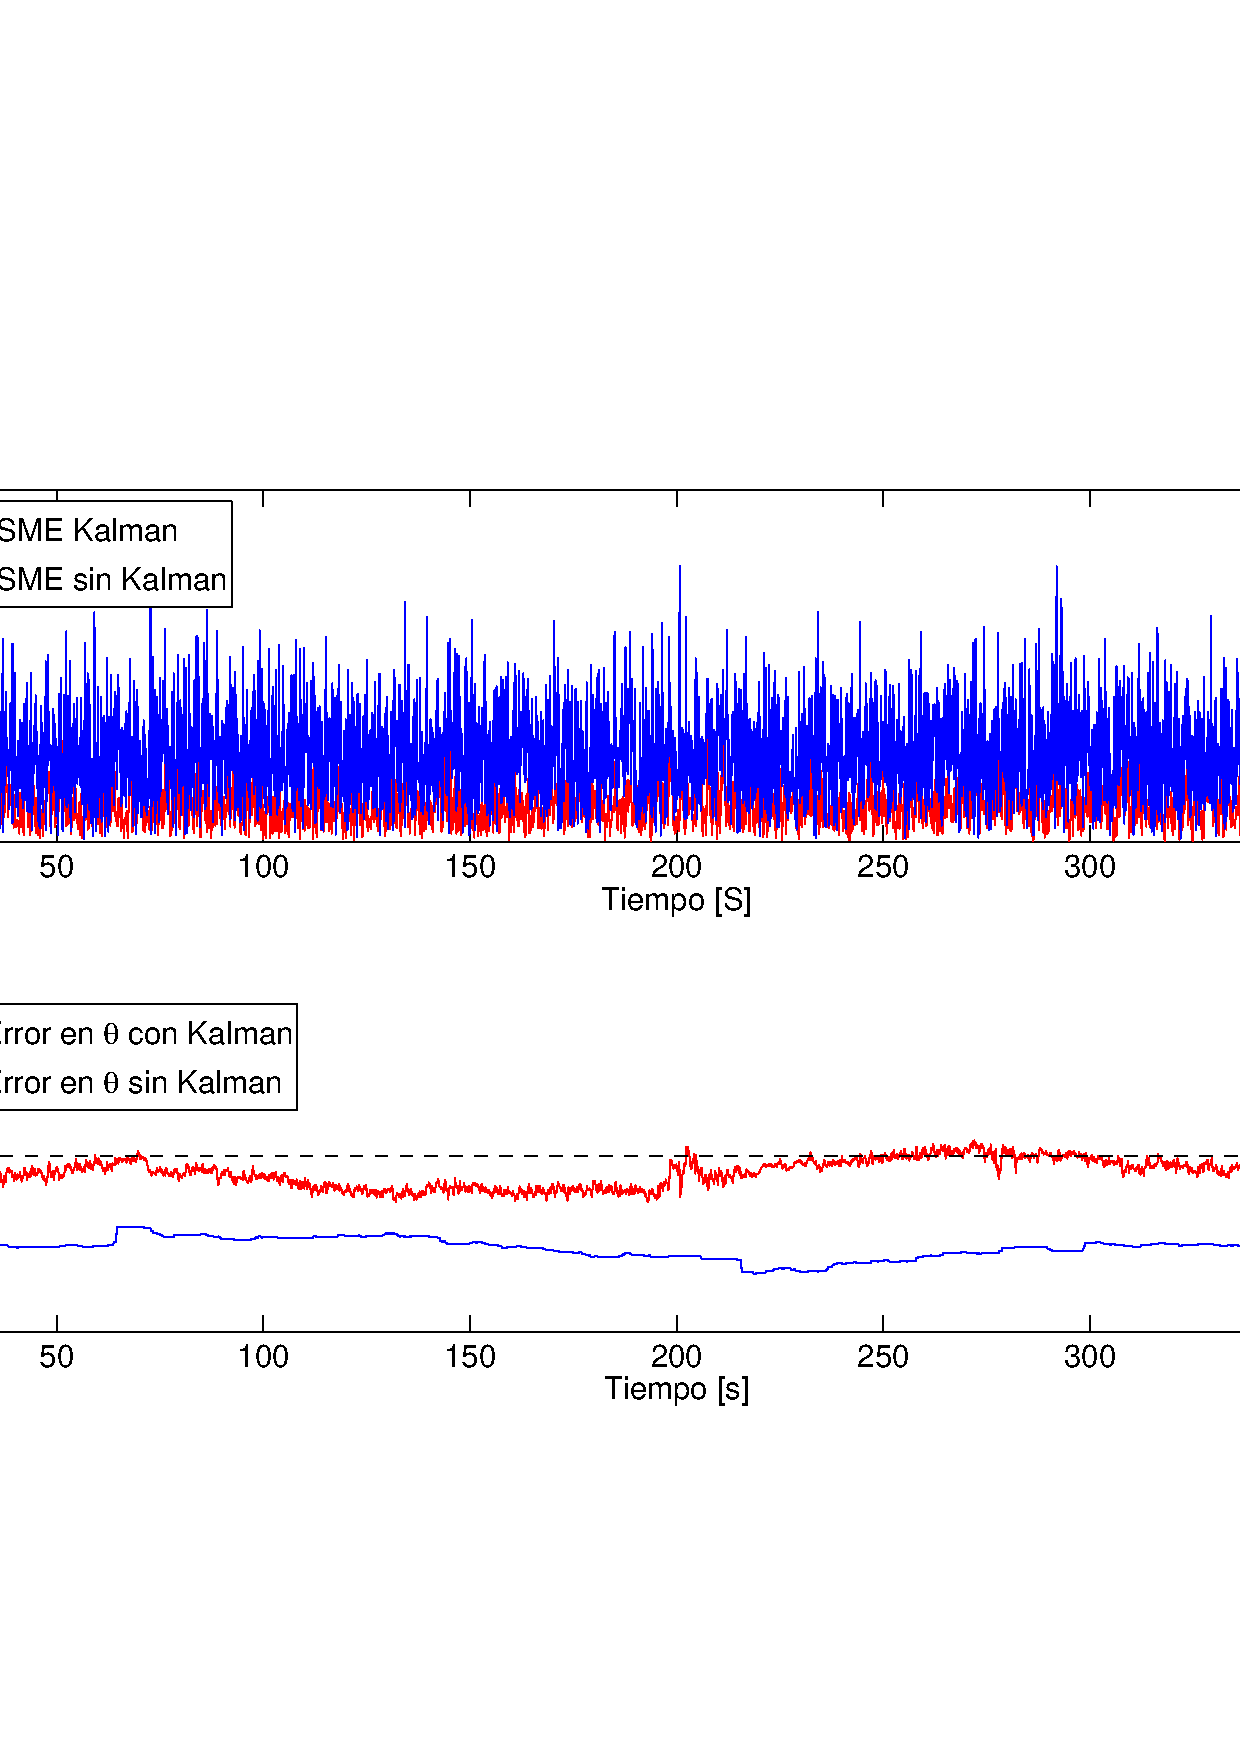
\includegraphics[width=.9\linewidth]{Imgs/sme_Lyap.pdf}
%	     	\end{center}
%   		\end{figure}
%% 	\end{minipage}
%\end{frame}
%
%\section{Conclusiones}
%
%\begin{frame}
%  \frametitle{Conclusiones}
%  \begin{itemize}
%  \item Se consigue la convergencia a la trayectoria con ambas estrategias y el EKF.
%  \item Se muestra la convergencia del estimador basado en EKF en ambos casos.
%  \item El EKF cumple su función de estimador y filtro en el sistema no lineal.
%  \item El control basado en Lyapunov no consigue el seguimiento de trayectoria en ausencia del EKF.
%  \item La variable no medida afecta en menor medida a la estrategia numérica.
%  \end{itemize}
%\end{frame}
%\begin{frame}
%\Huge{\centerline{¡Gracias!}}
%\end{frame}

\end{document}

%%% Local Variables: 
%%% mode: latex
%%% TeX-master: t
%%% End: 







